\documentclass{article}
\usepackage[UTF8]{ctex}
\usepackage{geometry}
\usepackage{natbib}
\geometry{left=3.18cm,right=3.18cm,top=2.54cm,bottom=2.54cm}
\usepackage{graphicx}
\pagestyle{plain}
\usepackage{float}	
\usepackage{setspace}
\usepackage{caption2}
\usepackage{datetime} %日期
\renewcommand{\today}{\number\year 年 \number\month 月 \number\day 日}
\renewcommand{\captionlabelfont}{\small}
\renewcommand{\captionfont}{\small}
\begin{document}

\begin{figure}
    \centering
    
\includegraphics{upc.jpg}

    \label{figupc}
\end{figure}

	\begin{center}
		\quad \\
		\quad \\
		\heiti \fontsize{45}{17} \quad \quad \quad 
		\vskip 1.5cm
		\heiti \zihao{2} 《计算科学导论》课程报告
	\end{center}
	\vskip 3.0cm
		
	\begin{quotation}
% 	\begin{center}

		\doublespacing
		
        \zihao{4}\par\setlength\parindent{7em}
		\quad 


		学生姓名:\underline{\qquad  万正浩 \qquad}

		学\hspace{0.61cm} 号:\underline{\qquad 1907030128\qquad}
		
		专业班级:\underline{\qquad 本研一体班(人工智能类) \qquad  }
		
        学\hspace{0.61cm} 院:\underline{计算机科学与技术学院}
% 	\end{center}
		\vskip 3cm
		\centering
		\begin{table}[h]
            \centering 
            \zihao{4}
            \begin{tabular}{|c|c|c|c|c|c|c|}
            % 这里的rl 与表格对应可以看到,姓名是r,右对齐的;学号是l,左对齐的;若想居中,使用c关键字。
                \hline
                课程认识 & 问题思考 & 格式规范 & IT工具 & Latex附加 & 总分 & 阅卷老师 \\
                30\% & 20\% & 20\% & 20\% & 10\% &  &  \\
                \hline
                 & & & & & &\\
                & & & & & &\\
                \hline
            \end{tabular}
        \end{table}
		\today
	\end{quotation}

\thispagestyle{empty}
\newpage
\setcounter{page}{1}
% 在这之前是封面,在这之后是正文
\section{引言}
通过一学期的对于《计算科学导论》的学习,我在计算科学方面受益匪浅。\par
计算科学是对描述和变换信息的算法过程,包括对理论分析、设计、效率、实现和应用等进行的系统研究。全部计算科学的基本问题是,什么能(有效地)自动进行、什么不能(有效地)自动进行。本科学来源于对算法理论、数理逻辑、计算模型、自动计算机器的研究,并与存储式电子计算机的发明一起形成于20世纪40年代初期。\par

同时我在其中的AR领域进行了较为深入的研究,并通过演讲和提问的形式得到老师的指导。\par

\section{对计算科学的认识和体会}
计算科学的研究包括了从算法与可计算性的研究到根据可计算硬件和软件的实际实现问题的研究。这样,计算科学不但包括从总体上对算法和信息处理进行研究的内容,也包括满足给定规格要求的有效而可靠的软、硬件设计——它包括所有科目的理论研究实验方法和工程设计。计算科学所有分支领域的根本任务是进行计算,其实质就是字符串的变换。
另外,计算科学的分支学科是构造性数学基础、计算的数学理论、计算机组成原理、器件与体系结构、计算机应用基础、计算机基本应用技术、软件基础和软件开发方法学。发展计算科学各个分支学科的目的有两个:一是针对各种实际问题应用背景的特点,希望能够不断地制作出性能更好的计算机系统。另一个是针对计算机在各行各业中的各类具体应用,为了在计算机系统上更有效地进行科学计算和事务处理,也必须首先发展支持计算机具体应用的各种共性思想、共性理论、共性方法和共性技术。而计算科学的三个基本的学科形态是理论、抽象、设计。理论是数学科学的根本;抽象(模型化)是自然了些的根本;设计是工程的根本。\par

计算科学的知识组成结构由早期对计算科学研究的计算模型、计算机设计、高级语言和科学计算,转向计算科学蓬勃发展的时期的如形式语义学、软件开发方法学等一大批理论、方法和技术。这一时期的两个显著特点,一是学科研究和开发渗透到社会生活的各个方面,广泛的应用需求推动了学科持续高速发展,一是经过大量的实践,人们开始认识到软件和硬件之间有一个相互依托,互为借鉴以推动计算机和软件发展的问题。从上世纪80年代起,针对集成电路芯片可预见的设计极限和一些深入的研究中所遇见的困难,开始认识到学科正在走向深化。图形学和图像处理这两个方向的迅速发展不仅使计算机的各种应用变得易于为社会接受,而且随着计算机硬件和数据库技术的进步,计算机应用触及到了一些以前被认为是较为困难的领域,并引发了计算集合、多媒体技术、虚拟现实等计算可视化方向的发展。\par

最终,计算科学的知识组成结构分成三个层面。第一层面是计算科学的应用层,包括人工智能应用与系统,信息、管理与决策系统,移动计算,计算可视化,科学计算等计算机应用方向。第二层面是计算科学的专业基础层,是为应用层提供技术和环境的一个层面,包括软件开发方法学,计算机网络与通信技术,程序设计科学,计算机体系结构,电子计算机系统基础。第三层面是计算科学的基础层,它包括计算机的数学理论,高级逻辑等内容。随着科技逐步发展,拓展和提高计算机的应用领域和应用水平这两个目标使学科的发展形成了三条相对独立的主线,分别是计算模型与计算机,计算模型、语言与软件开发方法学,应用数学与计算机应用。\par

\subsection{针对计算科学的深入理解}
科学家在科学的研究过程中实际上涉及到科学发现、科学推理和工作的方式方法问题,是科学方法论的中心问题,这个问题有三个方面:如何开店研究的对象?如何发现新的知识和如何证明信知识的真实性?发现和证明新知识应该依据什么推理规则?因此,计算科学科学家的研究方法分为以下几步,在进行科学研究时,首先要认识到问题的存在;要把问题的非本质方面找出来,加以剔除;要把能够找到的、同这个问题有关的全部数据都收集起来;进行假设或假说;对以前未打算进行的实验的结果作出推测;如果实验获得了预期的结果,那么假说便得到了强有力的事实依据,并可能成为一种理论,甚至成为一条“自然定律”。但也有极少数的像凯库勒领悟到苯的化学结构那样幸运的发现,不必按部就班。\par

\subsection{计算科学发展历史}
由古至今,计算科学就在人们的生活中起到一定的作用,而且是越来越重要的。古代人民已经懂得以物易物,发展到后来用货币,价格的多少、汇率都用到了计算,就是最原始的计算科学。不管是3000年前的欧几里德算法(辗转相除法),还是一千多年前的祖冲之的圆周率、南宋的秦九韶算法,还是时至今天的高速发展的科技,一切都是出于人类的需要和不断地探索。人类是需要计算科学的。\par

近年来,计算科学已经渗入到各个领域——生活、工作、政治。文化、环境、经济以及军事。由于计算机科学技术的迅速发展,特别是网络技术和多媒体技术的迅速发展,计算机不断地拓展新的应用领域。通信技术与计算机技术的结合,产生了全球卫星定位系统(GPS),地理信息系统(GIS);多媒体技术的发展更是如日中天,在音乐、舞蹈、电影、电影、电视和娱乐、虚拟现实、辅助设计、辅助教学中得到了广泛的应用。计算科学的发展势头不容小觑,特别是已经触及到了经济和军事,利比亚战争就是一个很好的例子,稍加以运用就能摧毁一方。中国作为发展中国家,发展经济是离不开科技发展的,而这方面的发展更有赖于中国的计算机科学与技术专业等人才培养。\par


\section{对演讲主题AR技术的研究}

\subsection{AR技术现存的技术问题}
1、硬件限制\par

ARKit和ARCore都寄希望于硬件厂商未来发布的手机上,这就意味着,有大量的消费者将被排除在外,除非他们升级自己的硬件。目前谷歌和苹果的解决方案都不是跨平台的,所以开发人员不得不从苹果切到安卓,或者从安卓跳到苹果,以满足大多数用户的需要。\par

2、你仍需要一个应用程序\par

ARKit和ARCore都集成到设备的操作系统中,这使得它们与那些只在系统上一层的第三方软件相比,拥有更强大的性能。但是,包含内容和体验的代码仍然需要通过应用程序来下载。事实上,开发一个App只是冰山一角 ,如何把App推销出去才是更艰巨的任务。\par
3、没人想体验功能单一的产品\par

为了让自己的应用看起来值得下载,开发人员应避免任何功能单一的体验。就算你能创作出一段世界上最酷炫的动画,但在反复观看后,它也会变得很无聊。\par

想要做出好的内容,你可能需要问自己这些问题:用户在第一秒可以做什么?在第一分钟能做什么?在第一天和第一周呢?体验不能一成不变,你得确保它们能不断升级。除了让内容更有深度外,解决这个问题的唯一办法,就是提供一个动态的解决方案,每次都有所不同。\par

以《TheMachines》为例,它是通过多人协作这个方案,让游戏即使没有新的内容也依然值得玩。\par

4、昂贵的3D\par

预算通常是“梦想杀手”,对AR和MR而言,大部分预算被用来创造3D的东西。客户端要么没有真正可用的3D设备,要么没有可用的格式。如果要将电影/VFX分辨率或CAD制造文件,转换成可以在消费者移动手机里使用的3D内容,这是一项极大的工作量。而且,所需的3D 数量也是个问题。\par

正如前面提到的,内容的丰富性很重要。例如,演示一张咖啡桌很简单,但如果某个品牌要展示数百种产品,又该怎么办呢?IKEA Place App就是一个很好的例子,它集合了大量的3D对象,据说目前已经有超过2000个品目可以AR展示。\par

5、位置的限制\par

有一个原因可以解释为什么这么多的ARKit Demos是在开阔的地方演示的。由于ARKit和ARCore无法检测或解决,使得碰撞和遮挡成为一个重大的问题。细心对比的话,我们会发现,一个在广阔空间看起来很棒的演示,如果在咖啡厅或在课堂上演示,看起来就像被破坏了。\par

当位置发挥作用时,就有更多的因素需要考虑进来,这会很不一样。我们不得不面对快餐桌尺寸,零售商理想的客流量,主题公园的照明条件改变甚至地标上的磁性干扰等等。\par

例如计算机无法明确区分地面,桌面与墙面的区别,在计算机“眼中”,这些都属于平面,甚至是可以无限延展的平面。因此,AR通过计算机视觉达到对事物的理解是一大突破口。\par
\begin{figure}[h]
	\centering
	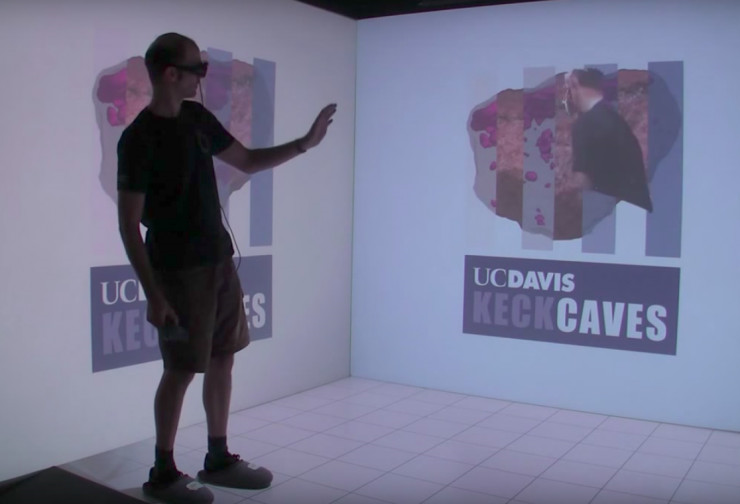
\includegraphics[scale=0.4]{AR1}
	\caption{AR设备产生的视场角}
	\label{fig1}
\end{figure}\par\begin{figure}[h]
	\centering
	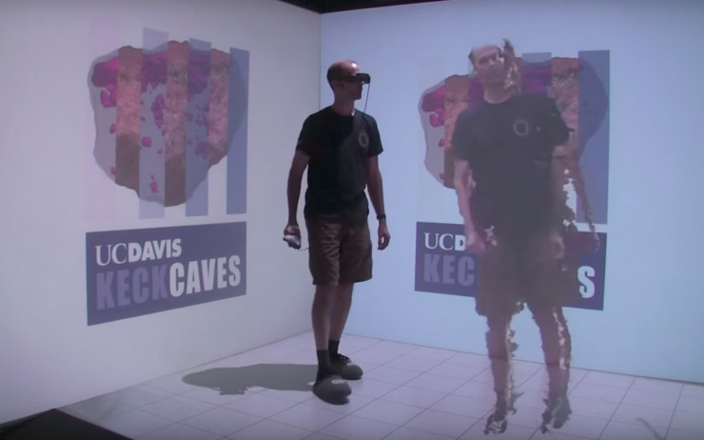
\includegraphics[scale=0.4]{VR1}
	\caption{VR设备产生的视场角}
	\label{fig2}
\end{figure}\par
同样,与VR技术相比,AR在显示器中能够呈现的视场角非常小。什么是视场角呢?就是图像能在用户眼中呈现的角度范围。视场角的大小与肉眼视野如果越相近,那么显示器的效果就越加优越。否则,使用AR设备,用户会认为他们使用的是望远镜,视野太有限。如果大脑就无法通过直观的映射将 AR 世界看作真实世界的一部分,所谓的沉浸感也会化为乌有。由于VR完全是基于虚拟场景,所以,对于显示器呈现影像没有太大的视场角限制。但是AR是基于摄像头的,也就是说,要让AR显示器呈现图像的视场角增大,必须同时增大摄像头的视场角。并且也需要同时考虑 Tom Caudell 和 David Mizell指出的,“要使得虚拟世界和真实世界更好地结合,对于增强现实的定位技术的要求在不断增强。”因此,第二个问题就是扩大摄像头与显示器的视场角,并且增强AR的定位和角度测量能力。\par

AR的自适应设计:AR自适应设计的目的是使AR涵盖跨越三维空间的任意环境,尤其是快速适应一些先前未映射的场景,并进行虚拟图像的处理。有一个非常经典的例子,制作一款结合AR技术的射击游戏。要求游戏中的NPC从特定房间中钻出来,并且与用户进行实时互动。但是,如果AR系统不预先对环境进行映射处理,AR系统连屋子里可能有另一个房间都不知道。因此,实现AR的自适应设计有助于增强AR系统的现实性,也是使其能够实现更加长效更加实用更加广泛深远影响的点睛之笔。\par

\subsection{对于现存问题的分析}
首先还是探讨一下AR系统对于物体的理解这一问题。如果单纯要让计算机通过摄像头识别和理解一个三维物体是非常困难的。
又比方说,计算机可以通过摄像头获取一个啤酒瓶的图形信息,但是它难以探测到酒瓶内部还有大量空间,即无法理解酒瓶。更例如,计算机无法理解酒瓶之中的啤酒平面无法高于瓶口所在的平面,树根不会长在天上,树叶不可能长在泥土里面。所以如果需要达到理解物体的目的,就需要较为庞大的理解算法体系,不仅对程序员是一种挑战,而且也无法达到“超越”人类智慧,真正达到人工智能的目的。那么,对于计算机理解物体这一步,就必须用到计算机的深度学习来构建计算机神经网络。\par

AR成像的关键设备是头戴式AR显示眼镜,它是通过将屏幕上现实的画面投射到用户眼中来实现信息输出的。但是往往该类设备体积与质量较大,不适于头戴,而如果缩小显示设备体积,那么其视场角也会随之减小。Oculus此前表示,想实现真正的沉浸感,视场至少要达到 90 度,因此 AR 必须尽快翻过这座大山。不论是AR还是VR,对于头戴式显示器的最大要求就是用户体验的沉浸感。就像如今影院的屏幕,越来越趋向大屏(即增大视场角)和imax,用来增加观影人的沉浸式体验。但是如同我们所知道的,AR显示器的成像是基于摄像头获取的图像信息,所以,扩大头戴设备视场角的一大关键也就是如何扩大其摄像头的“视野”。\par

另外,就是计算机角度计算的问题。前些天我看到一个短视频,就是运用AR技术,将摄像头获取的人脸上附上猫脸的图,但是问题来了,当人的头低下俯视到一定程度时,计算机附上的猫脸就无法呈现了,它无法随着人脸角度的转变而转变图像。所以,我认为,这依旧需要使计算机对物体充分理解,让计算机明白,虽然人的脸俯下了,但依旧是人脸的一部分,依旧可以将虚拟图像即AR技术进行运用。\par

最后就是要分析AR自适应设计的问题了。就是说怎么样才能在现有设备的基础上,通过对计算机软件的改进,使其对先前未进行映射的物体快速做出反应。就还是比如说现实场景的射击游戏吧,首先是要靠计算机视觉和深度学习,对房间、墙面、门进行理解和快速反应,如果能做到看见即理解,理解即映射,那么,或许可以说是AR自适应设计的一个突破了。\par

\subsection{对计算机视觉以及计算机神经网络的理解}
计算机视觉是一种通过摄像头模拟人眼,并用计算机的算法模拟人类大脑并进行结合的生物视觉模拟技术。与AR类似,计算机视觉的最终目的是使计算机能像人和其他生物一样通过视觉观察理解世界,由此具有自己能够适应环境的能力。而AR技术,就是计算机视觉的一个应用和表现形式。\par

计算机神经网络,就是仿生人类大脑,从而构建起的具有判断、适应、决策能力,可以同时处理很多类型数据的算法体系。我们所说的计算机深度学习,就是构建计算机神经网络的大量神经元,以完善计算机处理事物的能力。先前所说的理解物体的能力,就是计算机神经网络的分支。\par

\subsection{对于AR设备即技术改进的思考}
以上发觉的问题可归为:

1、如何改进或者研发更加新型的AR设备,以使其在扩大视场角的同时不增加其体积和质量。

2、如何将计算机视觉与计算机神经网络和AR的自适应设计相连接并使之完善。

由于AR的虚拟影像的呈现是需要计算机的处理来实现的,但是又无法将整一台计算机戴在头上,所以需要研发一款体积小并且具有较强的图形处理系统的芯片。众所周知,如同笔记本一样,既要满足高性能,又要实现低散热是一件非常困难的事情,所以对于研发该芯片还要考虑散热问题。而先前的较大体积AR设备主要问题并不是视场角不足,而是达到了可以实现沉浸式的设备处理器过大,体积过大。所以,研究一宽兼备散热小,体积小且性能高的芯片是成功推出便携,顺畅,优质的头戴AR设备的必经之路。\par

而说到将计算机视觉和神经网络与AR相结合这一问题,还是要训练出如同阿尔法狗这样的,可以对于棋盘上任意棋子摆放行为进行快速且最优化处理的神经网络。虽然棋子的摆放排列可以计算到无穷无尽的树木,但它终究是有局限的,而实地场景需要计算机考虑到的实物数据类型、计算思考方式要比下赢一盘棋复杂得多得多。\par
\subsection{AR的应用及市场方向}
从宏观来看,AR整体市场逐渐趋向利好,早起受限于计算机计算能力不足、图形显示效果差的影响,长期处于技术摸索和突破的阶段。但自从今年起苹果和安卓两大移动平台直接支持,行业将逐渐向消费级市场发展。不过也要看到,当前的市场还处于初级阶段,消费级市场用户对AR的了解程度仍然很低,而且当前计算能力和图形显示效果仍然不能达到我们预想的要求,真正的行业拐点仍需较长时间。我们通过几个数据来看下当前环境。\par
2016年第四季度,全球AR设备销售量仅有4.8万台。\par

2016全年AR设备的总营收为2.09亿美元,不过在2021年设备有望突破487亿美元。\par

VR设备在2016年的总营收为21亿美元,预计在2021年会增长到186亿美元。\par

AR/VR 目前总发货量为1010万台,2016营收为52亿美元,预计2021年总发货量有望超过9940万台。\par
不过,从长远来看,AR/MR将有更好的市场前景,预计终将取代智能手机。但因技术限制和市场认可度较低,短期内销量仍然很低,预计在2025年有可能和智能手机销量打平手。\par

而新兴的AR/MR,在消费级市场普遍落后VR18-24个月,目前主要瞄准企业级市场。\par
针对AR市场,由于硬件价格高昂,短期内利润很低,但长期看,在拐点之后生产成本将大幅度下降,同时提供更多的利润空间;而在软件市场,凭借各大互联网平台的深耕,也将在各自的领域实现大规模增长。整体市场达到900亿美元,其中接近一半来自硬件。\par
通过与VR行业的对比,能够更好的看出AR行业发展的情况及预期。\par

对于整体市场发展,各家均对当前市场及短期内趋势的判断,主要有以下三点:\par

1.当前市场仍处于初级阶段。各家对短期内爆发均持较为谨慎的态度,普遍预爆发拐点在2020年甚至之后。大平台级的市场,行业内对爆发有一个预估值,普遍要达到亿级销量才有可能迎来爆发。目前看AR市场如果不考虑依托苹果和安卓的移动设备,硬件达到亿级销量十分遥远。而软件市场更多的集中在工业领域,消费级市场游戏为主,且需有大IP加持,如Pokemon Go这种,尚未出现killer app。\par
2.大平台带动对产业发展有积极意义。通过以上各公司近一年半数据变化可以看出,大平台的进入直接带动整体市场风向的变化。在两大平台推出相关SDK前,研发主要集中在第三方SDK,如Vuforia、ARToolKit、视+、亮风台等,产品主要以企业定制的应用和展示型demo为主(Pokemon Go是特例),媒体宣传多为个案,没有形成趋势,也未在社交网络爆发。苹果和Google的相继进入,虽然在运行AR的设备和系统上都有要求,但仍然无法阻挡在社交媒体上引起一阵风潮,也引得投资界及整个市场重新将关注点投向AR市场。两大移动平台的竞争进一步推动整个产业发展,对市场短期预测发生了根本性转变,从VR为主,转变为AR为主,且移动AR占据主导。\par
3.移动AR是短期内主要发展趋势。根据智能手机操作系统的统计数据显示,iOS和安卓已经占据整个移动市场的99%。\par
\bibliographystyle{plain}
\bibliography{1}


\maketitle

\section{总结}
对于此次课程来说,计算科学导论的开设极大地开阔了我的知识面,在对我的相关专业得到更进一步的认识的同时,让我对未来的研究方向更加明确,为自己以后研究生和博士时期的探索指明了方向,可谓具有指向标式的作用。\par
而对于此次报告而言,只是我对于AR方面的一个非常浅显的言论,但是,兴趣是最好的老师,通过对相关专业的兴趣,能支持我在未知的领域不断探索,探究现在还未发现的一些奥秘,正如前文中所提及的,在这个领域的发展尚且还有许许多多不足之处,换言之,便是还有许许多多未知的领域等着我去探索,还有许许多多的问题等着我去解决,通过对一个领域的探索,我们往往能发现许多光明的大陆。\par 


\section{附录}
\begin{itemize}
    \item 申请Github账户,给出个人网址和个人网站截图\par 
    https://github.com/Alex-star-arch/Alex-star\par 
    \begin{figure}[H]
    	\centering
    	
\includegraphics[scale=0.6]{GitHub}
    	\caption{GitHub截图}\par
    	\label{fig:深度学习}
    \end{figure}
    
    \item 注册观察者、学习强国、哔哩哔哩APP,给出对应的截图\par 
    观察者:https://user.guancha.cn/user/personal-homepage?uid=720737\par
    \begin{figure}[H]
    	\centering
    	
\includegraphics[scale=0.6]{GCZ}
    	\caption{观察者截图}\par
    \end{figure}
学习强国:https://www.xuexi.cn/        \par 
   \begin{figure}[H]
	  \centering
	  
\includegraphics[scale=0.6]{XXQG}
	  \caption{学习强国截图}\par
   \end{figure}
哔哩哔哩:https://www.bilibili.com/\par 
\begin{figure}[H]
	\centering
	
\includegraphics[scale=0.6]{BLBL}
	\caption{哔哩哔哩截图}\par
\end{figure}
    \item 注册CSDN、博客园账户,给出个人网址和个人网站截图\par 
    CSDN: https://i.csdn.net/\par 
    \begin{figure}[H]
    	\centering
    	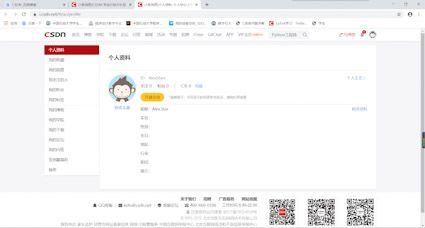
\includegraphics[scale=0.6]{CSDN}
    	\caption{CSDN截图}\par
    \end{figure} 
    博客园: https://home.cnblogs.com/u/1882481/ \par 
     \begin{figure}[H]
    	\centering
    	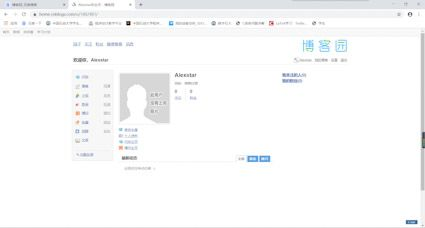
\includegraphics[scale=0.6]{BKY}
    	\caption{博客园截图}\par
    \end{figure} 
    \item 注册小木虫账户,给出个人网址和个人网站截图 \par 
    小木虫:http://muchong.com/bbs/space.php?uid=19942043 \par 
    \begin{figure}[H]
    	\centering
    	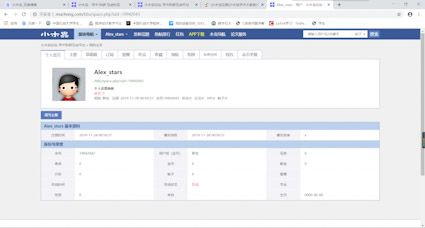
\includegraphics[scale=0.6]{XMC}
    	\caption{小木虫截图}\par
    \end{figure} 
\end{itemize}


\hspace*{\fill} \\


\bibliographystyle{plain}
\bibliography{references}


\end{document}
